% FTEC5660 Reproducibility Work -- LaTeX report
% Typeset to match the style of the assignment brief:
% article / 11pt / Computer Modern / US Letter / 0.8in margins /
% Name + Student ID header / centred bold course title with rule /
% numbered bold sections / centred page numbers.
\documentclass[11pt,letterpaper]{article}
\usepackage[T1]{fontenc}
\usepackage[utf8]{inputenc}
\usepackage[margin=0.8in]{geometry}
\usepackage{graphicx}
\usepackage[hidelinks]{hyperref}
\usepackage{xurl}
\usepackage{amsmath}
\usepackage{booktabs}
\usepackage{array}

\graphicspath{{figures/}}
\setlength{\parindent}{0pt}
\setlength{\parskip}{4pt plus 1pt}
\setlength{\tabcolsep}{3pt}
\setlength{\emergencystretch}{1.5em}
\tolerance=1200
\newcommand{\code}[1]{\texttt{\detokenize{#1}}}
\newcommand{\lcode}[1]{\url{#1}}
\urlstyle{tt}
\pagestyle{plain}

\begin{document}

\noindent
\begin{tabular}{@{}p{4.5in}@{}l@{}}
Name: JIANG Jiawei & Student ID: 1155271183
\end{tabular}

\begin{center}
\textbf{Agentic AI for Business and FinTech (FTEC5660)}\\[3pt]
Reproducibility Work: ToolTree bidirectional pruning \quad Due date: 13 November, midnight.\\
\vspace{2pt}
\rule{\linewidth}{0.4pt}
\end{center}

\vspace{2pt}

\section*{Abstract}

This report reproduces a clearly scoped, mechanism-level claim of \emph{ToolTree:
Efficient LLM Agent Tool Planning via Dual-Feedback Monte Carlo Tree Search and
Bidirectional Pruning} (ICLR 2026). The official repository was cloned, installed
and executed. Its shipped 32-test behaviour suite passes, and three behaviours with
explicit numeric assertions were re-measured independently: all reproduce exactly.
To quantify the paper's central efficiency claim---that bidirectional pruning
concentrates the computational budget on promising tool chains---I built a
controlled, fully offline instrument of 24 synthetic tool-planning tasks with known
gold plans, driving the \textbf{unmodified} upstream MCTS with the deterministic
stubs that the repository itself ships for its tests. A single isolated
modification, disabling post-evaluation pruning by changing \code{tau_post} from
0.4 to 0.0, was then measured over five paired seeds (240 searches). Removing
post-pruning increased post-evaluation calls by 57.9\% (25.33 to 40.00 per run),
tree nodes by 91.3\%, planner calls by 109.6\% and wall time by 74.8\%, while
collapsing plan success from 0.983 to 0.133 and tool F1 from 0.994 to 0.635.
Every run without post-pruning exhausted the 40-rollout budget; 88 of 120 baseline
runs terminated early by tree exhaustion. I also found that the shipped
early-stopping default masks most of this effect, which is reported as a hidden
assumption and verified with a sensitivity protocol. The paper's headline
benchmark numbers are \textbf{not} reproduced and are explicitly out of scope:
the release ships no benchmark data and requires a live LLM for three separate
roles. Because the underlying LLM is replaced by deterministic stubs,
\textbf{results are not directly comparable to the paper}.

\section{Project Summary and What I Tried to Reproduce}

ToolTree is an agentic planning system: given a user query and a tool set, it plans
a multi-step tool trajectory using Monte Carlo Tree Search. Each candidate tool
call is scored \emph{before} execution (pre-evaluation) and \emph{after} execution
(post-evaluation); branches scoring below \code{tau_pre} and \code{tau_post} are
pruned. The surviving highest-value trajectory is returned as the plan. This is a
genuine multi-step, tool-using agent loop rather than a single prompt-response,
and it satisfies the eligibility checklist: public GitHub repository with a
runnable pipeline, a documented claim with an evaluation script, and a subset that
runs on a laptop.

\textbf{Target claim (chosen early).} The upstream README states that bidirectional
pruning works by ``eliminating unpromising branches, concentrating computational
budget on promising tool chains'', and the release ships a 32-test behaviour suite
pinning search-termination and pruning invariants. The paper additionally reports
roughly a 10\% average gain over baselines across four benchmarks and an efficiency
advantage in Figure~3. Following Section~2 of the assignment, I selected
\textbf{one small target}: the budget-concentration mechanism and the repository's
pinned numeric behaviours. The four-benchmark headline accuracy is deliberately
not attempted.

\textbf{Why this scope is legitimate.} The upstream README states plainly: ``This
repository ships no benchmark data; download each from its official source''.
Running GTA, m\&m, ToolBench or RestBench therefore needs multi-GB dataset
downloads plus a live OpenAI-compatible endpoint for the planner, the dual judge
and the answer predictor. The assignment explicitly permits both (i) reproducing
one small, clearly defined experiment and (ii) replacing a deprecated/hard-coded
LLM with an accessible model, provided the change is documented as a controlled
variable. I go one step further on the cost axis and use the deterministic stubs
already shipped in the upstream test suite, so the study needs no API key, no
network access at run time, and can be re-run bit-for-bit by the grader.

\textbf{Comparability statement (required by the assignment).} The underlying LLM
differs: planner, judge and answer-predictor are replaced by deterministic stubs,
not by DeepSeek or the paper's original model. \textbf{Results are not directly
comparable to the paper because the underlying LLM differs.} All comparisons in
this report use the same tasks, the same evaluation metrics (the repository's own
\code{tool_f1} / \code{plan_f1}), the same harness and paired seeds, so the
baseline-versus-modification comparison is internally fair.

\section{Setup Notes (Environment, Data, Keys, Compute)}

\begin{table}[htbp]
\centering\small
\begin{tabular}{@{}p{0.17\linewidth}p{0.80\linewidth}@{}}
\toprule
\textbf{Item} & \textbf{Value / decision}\\
\midrule
Upstream code & \url{https://github.com/SYang2000/ICLR_2026_ToolTree}, cloned at
commit \lcode{fed7a608ca54ba2e75078f9a1f409c9aa7fab18f} (2026-07-05), imported
unchanged as the first commit of this fork. Original README preserved at
\code{docs/UPSTREAM_README.md}.\\
Environment & Python 3.13.14, Windows 11 (10.0.26200), git 2.55.0.windows.3.
Dependencies: upstream \code{requirements.txt} (openai, pyyaml, numpy) plus
pytest 9.2.0 and matplotlib 3.11.2.\\
Data & 24 deterministic synthetic tool-planning tasks in \code{repro/tasks.py}:
4 families (clean / trap / noisy / deep) $\times$ 6 variants. Each task has an
explicit gold tool chain, 5--7 tool cards and fixed pre/post evaluation scores.
No external dataset is downloaded.\\
Keys / network & \textbf{No API key, no secret and no network call at run time.}
The LLM boundary is replaced by deterministic stubs adapted from
\code{tests/test_tier1_fixes.py} (``Pure stubs -- no LLM server needed''). With a
real OpenAI-compatible endpoint, \code{enable_thinking_toggle} must be
\code{false} (see \code{src/llm/client.py}).\\
Compute & 240 searches (24 tasks $\times$ 5 seeds $\times$ 2 conditions) plus 240
sensitivity searches; total measured search time about 3.2 seconds of CPU work
(mean 4.9--8.5 ms per search). Entire pipeline finishes in under a minute on a
laptop; no GPU.\\
Hyperparameters & \code{tau_pre=0.3}, \code{tau_post=0.4},
\code{exploration_constant=1.4}, \code{max_rollouts=40}, \code{top_k=5},
\code{max_depth=4}. The first four match the meta block of the repository's own
logged demo run (\code{docs/static/demo_data.js}, seed 42).
\code{early_stop_patience=100} is a measurement-protocol choice applied
identically to both arms (justified in Section~5.1).\\
Seeds & 5 paired seeds. Gaussian jitter ($\sigma = 0.03$) is applied once per run
to each tool's pre/post score, clipped to $[0,1]$; the global RNG used by the UCT
tie-break is seeded from the same paired seed. Baseline and ablation therefore
see identical noise and tie-break randomness.\\
\bottomrule
\end{tabular}
\end{table}

\section{Reproduction Targets and Metric Definitions}

\subsection{Target A --- reported/pinned behaviours}

The upstream README claims a ``Behavior test suite (32 tests)'' and the release
notes describe fixes with explicit numeric assertions. I re-instantiate three of
those scenarios (\code{repro/verify_claims.py}) and record my own measurements,
so the report contains numbers rather than a bare pass/fail.

\subsection{Target B --- budget concentration (quantified)}

For each measured search I record plan quality and search cost:

\begin{itemize}
\item \textbf{Plan success}: 1 if the returned multiset of tools equals the gold
tool multiset, else 0. Upstream grades with multiset F1
(\code{src/evaluation/metrics.py}), which is order-insensitive; I follow that
convention. An order-sensitive \code{order_exact} field is kept as a transparent
secondary statistic, but not as the primary metric, because Eq.~1 gives unvisited
siblings an infinite UCT bonus and \code{MCTSNode.best_child} breaks ties
randomly, so tool \emph{order} is not a stable target.
\item \textbf{Tool F1 / Plan F1}: computed by the repository's own
\code{tool_f1()} and \code{plan_f1()} functions; multiset F1 over tool names and
over (tool, args) steps respectively.
\item \textbf{Gold-tool recall}: fraction of gold tools present in the returned
plan.
\item \textbf{Search cost}: pre-evaluation calls, post-evaluation calls (the
expensive LLM-judge calls), planner/argument-draft calls, rollouts used,
search-tree nodes created, post-pruned nodes and wall time in ms.
\item \textbf{Termination mode}: whether the search ended by tree exhaustion,
early stopping, or by hitting the 40-rollout budget cap.
\end{itemize}

All metrics are aggregated as mean $\pm$ standard deviation across the 5 seeds,
where each seed averages over the 24 tasks. Deltas are ablation minus baseline,
computed on paired seeds.

\section{Results: My Numbers versus Reported Numbers}

\subsection{Reproduction of the repository's reported behaviours}

\begin{table}[htbp]
\centering\small
\caption{Reproduction of reported/pinned behaviours. Reported values are the
upstream assertions/descriptions; measured values are produced by
\code{repro/verify_claims.py} on this machine. Raw transcript:
\code{repro/results/upstream_tests.txt}; JSON: \code{claim_verification.json}.}
\begin{tabular}{@{}p{0.29\linewidth}p{0.21\linewidth}p{0.29\linewidth}p{0.12\linewidth}@{}}
\toprule
\textbf{Claim (upstream source)} & \textbf{Reported} & \textbf{Measured here} & \textbf{Status}\\
\midrule
Behaviour test suite (\code{README.md}) & 32 tests pass & 32 passed in 1.34 s, exit code 0 & Reproduced\\
Exhausted search stops without revisit / re-backpropagation & 4 post-eval calls, 4 rollouts, root N = 4, root exhausted, best-Q history = 4 (budget = 50) & 4, 4, 4, True, 4 & Reproduced\\
A post-pruned branch is never rebuilt and re-judged & dead tool judged $\le 2$ times; 0 nodes with duplicate children & 2 judgments; 0 duplicate-child nodes & Reproduced\\
UCT selection follows Eq.~1 & UCT(a) $\approx 1.1594$, UCT(b) $\approx 1.3664$, UCT(b) $>$ UCT(a), best child = b & 1.1593, 1.3662, True, b & Reproduced\\
\bottomrule
\end{tabular}
\end{table}

The small UCT differences are floating-point rounding in the upstream comments,
not a discrepancy.

\subsection{Quantifying the budget-concentration claim}

Table~\ref{tab:main} compares the upstream configuration (post-pruning active)
with the modification (post-pruning removed). Every number is generated from
\code{repro/results/raw_runs.csv} by \code{repro/summarize.py}; no value is
hand-entered.

\begin{table}[htbp]
\centering\small
\caption{Main protocol. Mean $\pm$ s.d.\ across 5 paired seeds; each seed
averages 24 tasks (120 measured searches per condition). Delta = ablation $-$
baseline.}
\label{tab:main}
\begin{tabular}{@{}lrrrr@{}}
\toprule
\textbf{Metric} & \textbf{Baseline (ON)} & \textbf{Ablation (OFF)} & \textbf{Delta} & \textbf{Delta \%}\\
\midrule
Plan success (exact gold tool set) & 0.983 $\pm$ 0.020 & 0.133 $\pm$ 0.061 & $-$0.850 & $-$86.4\%\\
Tool F1 (upstream metric) & 0.994 $\pm$ 0.007 & 0.635 $\pm$ 0.046 & $-$0.359 & $-$36.1\%\\
Plan F1 (upstream metric) & 0.994 $\pm$ 0.007 & 0.635 $\pm$ 0.046 & $-$0.359 & $-$36.1\%\\
Gold-tool recall & 1.000 $\pm$ 0.000 & 0.693 $\pm$ 0.059 & $-$0.307 & $-$30.7\%\\
Returned plan length & 2.283 $\pm$ 0.041 & 2.500 $\pm$ 0.105 & +0.217 & +9.5\%\\
Pre-evaluation calls & 27.183 $\pm$ 0.531 & 53.067 $\pm$ 0.893 & +25.883 & +95.2\%\\
\textbf{Post-evaluation calls} & \textbf{25.325 $\pm$ 0.469} & \textbf{40.000 $\pm$ 0.000} & +14.675 & \textbf{+57.9\%}\\
Planner (arg-draft) calls & 35.833 $\pm$ 1.021 & 75.117 $\pm$ 1.523 & +39.283 & +109.6\%\\
Rollouts used & 25.325 $\pm$ 0.469 & 40.000 $\pm$ 0.000 & +14.675 & +57.9\%\\
\textbf{Search-tree nodes} & \textbf{27.408 $\pm$ 0.564} & \textbf{52.425 $\pm$ 0.533} & +25.017 & \textbf{+91.3\%}\\
Post-pruned nodes & 18.392 $\pm$ 0.276 & 0.000 $\pm$ 0.000 & $-$18.392 & $-$100.0\%\\
Wall time (ms) & 4.868 $\pm$ 0.262 & 8.511 $\pm$ 0.195 & +3.644 & +74.8\%\\
Best Q value & 0.484 $\pm$ 0.011 & 0.889 $\pm$ 0.003 & +0.404 & +83.4\%\\
\bottomrule
\end{tabular}
\end{table}

\textbf{Termination behaviour (the clearest evidence).} With post-pruning active,
88 of 120 baseline runs ended by tree exhaustion and only 32 hit the 40-rollout
cap. With post-pruning removed, \textbf{0 of 120} runs ended by exhaustion:
\textbf{all 120 hit the budget cap}. Post-pruning is therefore not merely a
quality filter---it is the mechanism that lets the search finish. Two further
observations: (i) the ablation's higher ``best Q'' (0.889 vs 0.484) is \emph{not}
a better plan, because with all branches kept alive the greedy final descent can
follow a high-value but semantically wrong chain; (ii) the quality collapse is
worst for the \code{noisy} and \code{trap} families (Table~\ref{tab:family}),
exactly where many admissible-but-unproductive distractors exist.

\begin{table}[htbp]
\centering\footnotesize
\caption{Per-family breakdown (main protocol, averaged over seeds and variants).
``deep'' tasks hit the budget cap even with pruning ON, because a 3-step gold
chain genuinely needs more search.}
\label{tab:family}
\begin{tabular}{@{}lrrrrrr@{}}
\toprule
\textbf{Family} & \textbf{F1 (ON)} & \textbf{F1 (OFF)} & \textbf{Post-eval (ON)} & \textbf{Post-eval (OFF)} & \textbf{Nodes (ON)} & \textbf{Nodes (OFF)}\\
\midrule
clean & 1.000 & 0.760 & 19.0 & 40.0 & 20.0 & 49.8\\
deep (3-step gold) & 1.000 & 0.720 & 40.0 & 40.0 & 45.0 & 54.3\\
noisy & 1.000 & 0.520 & 21.9 & 40.0 & 22.9 & 56.4\\
trap & 0.978 & 0.540 & 20.4 & 40.0 & 21.7 & 49.2\\
\bottomrule
\end{tabular}
\end{table}

\begin{figure}[htbp]
\centering
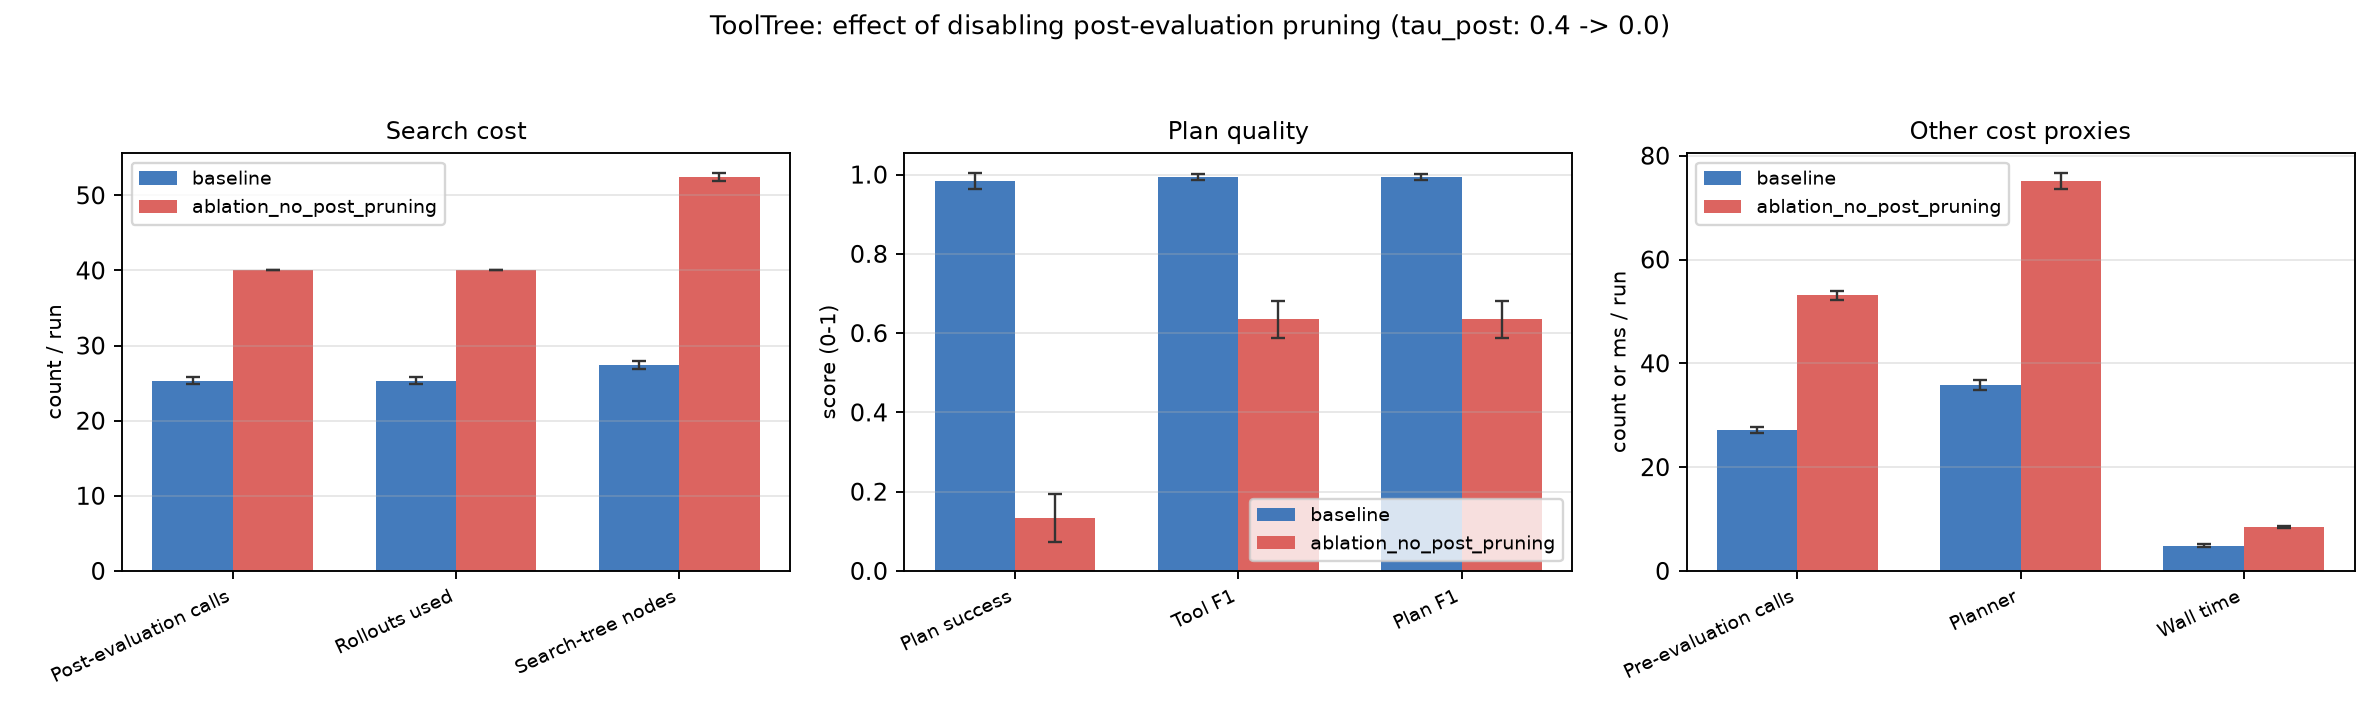
\includegraphics[width=0.98\linewidth]{figure_cost_quality.png}\\
\vspace{4pt}
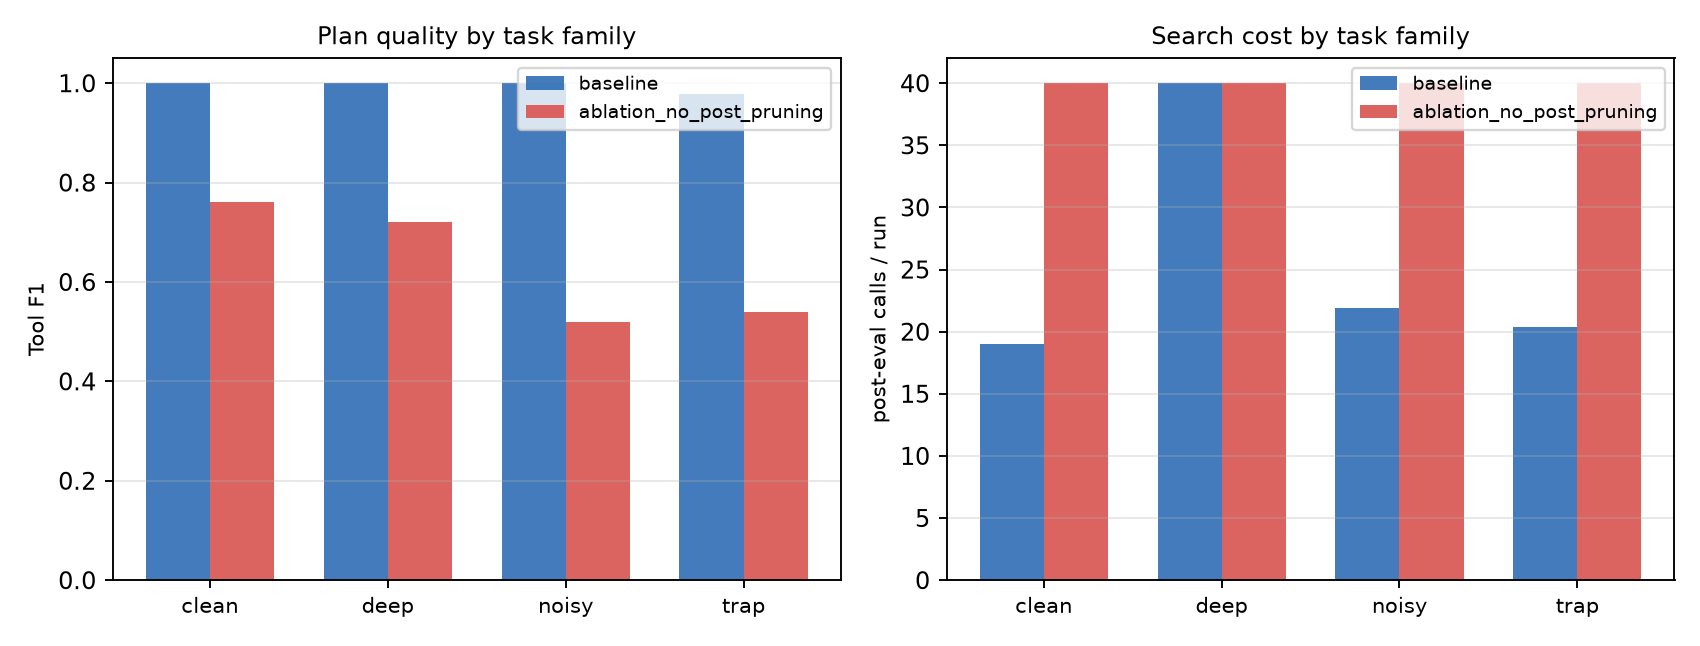
\includegraphics[width=0.76\linewidth]{figure_by_family.png}
\caption{Top: search cost, plan quality and other cost proxies, baseline vs
modification, with error bars across 5 seeds. Bottom: per-family plan quality and
search cost. Both generated by \code{repro/summarize.py}.}
\label{fig:results}
\end{figure}

\section{The Modification and Its Measured Impact}

\textbf{One isolated change.}
In \code{repro/configs/}, \lcode{ablation_no_post_pruning.yaml} differs from
\lcode{baseline.yaml} in exactly one value:
\code{mcts.tau_post} changes from 0.4 to 0.0. Because the post-evaluation reward
\code{r_post} is always non-negative, the pruning condition
\code{r_post < tau_post} can never fire, so post-execution pruning is disabled.
Pre-evaluation pruning, UCT selection, the MCTS loop, early stopping, the tool
manager, the judge, the planner, the tasks and the seeds are all unchanged. No
upstream source file is edited; the change lives in a single config file in its
own git commit (\code{7fd5b7a}). This satisfies the assignment's requirement that
the modification be isolated and measurable, and corresponds to the suggested
``ablation / parameter change'' category.

\textbf{Measured impact.} Roughly doubling the search cost (post-eval calls
+57.9\%, nodes +91.3\%, planner calls +109.6\%, wall time +74.8\%) while
destroying plan quality (plan success 0.983 $\to$ 0.133, tool F1 0.994 $\to$
0.635) is a large, unambiguous effect. It confirms the repository's
budget-concentration claim in the controlled setting, and additionally shows that
post-pruning is a \emph{correctness} mechanism here, not just an efficiency one:
the upstream \code{_get_best_trajectory} excludes post-pruned
(non-expandable) children from the final plan, so removing pruning also removes
that filter and lets low-value tools into the returned plan.

\subsection{Hidden assumption and sensitivity check: early stopping masks the effect}

An initial run with the shipped default \code{early_stop_patience=10} produced
almost no difference between the two arms (post-eval calls 11.90 vs 11.78; tool
F1 0.935 vs 0.904): both arms stopped after roughly 12 rollouts, before the
pruning difference could accumulate. Early stopping is therefore a
\textbf{confounder} for any cost measurement of this mechanism. Rather than
treating that as the modification, I raised \code{early_stop_patience} to 100
\textbf{in both configs} (a measurement-protocol choice, held constant across
conditions) and reran the shipped-default protocol as a sensitivity check
(Table~\ref{tab:sens}).

\begin{table}[htbp]
\centering\small
\caption{Sensitivity protocol: shipped early-stop default
(\code{patience=10}) applied identically to both arms. Under this setting the
pruning effect is largely hidden. Full table:
\code{repro/results/sensitivity_defaultstop/table_results.md}.}
\label{tab:sens}
\begin{tabular}{@{}lrrr@{}}
\toprule
\textbf{Metric} & \textbf{Baseline (ON)} & \textbf{Ablation (OFF)} & \textbf{Delta \%}\\
\midrule
Plan success & 0.675 $\pm$ 0.017 & 0.658 $\pm$ 0.055 & $-$2.5\%\\
Tool F1 & 0.935 $\pm$ 0.003 & 0.904 $\pm$ 0.028 & $-$3.3\%\\
Post-evaluation calls & 11.900 $\pm$ 0.208 & 11.783 $\pm$ 0.180 & $-$1.0\%\\
Search-tree nodes & 16.867 $\pm$ 0.135 & 17.700 $\pm$ 0.110 & +4.9\%\\
Wall time (ms) & 2.096 $\pm$ 0.100 & 2.223 $\pm$ 0.126 & +6.1\%\\
\bottomrule
\end{tabular}
\end{table}

\subsection{Other hidden assumptions identified}

\begin{itemize}
\item \textbf{Dataset availability.} The release ships no benchmark data; GTA /
m\&m require separate Hugging Face downloads, and the open-set ToolBench /
RestBench loaders raise \code{NotImplementedError} (``not supported in
step-by-step release'').
\item \textbf{Three LLM roles and endpoint compatibility.} Planner, pre/post
judge and answer predictor all call an OpenAI-compatible endpoint;
\code{src/llm/client.py} sends a vLLM-specific \code{extra_body} by default, so
non-vLLM endpoints (including DeepSeek) must set
\code{enable_thinking_toggle: false}.
\item \textbf{Plan-level vs real execution.} \code{tool_execution: mock} is the
default and scores plans without invoking tools; real execution needs the
backends in \code{src/tools/real_tools.py}. My study uses the shipped mock mode.
\item \textbf{Global RNG state.} \code{MCTSNode.best_child} uses
\code{random.random()} for tie-breaking, so unvisited siblings are explored in an
order that depends on global RNG state. My harness seeds it explicitly.
\item \textbf{One-shot expansion and top-K shortlist.} Expansion happens once per
node and only the top 5 survivors by \code{r_pre} are instantiated, so cost is
sensitive to \code{top_k} and to the number of admissible tools.
\item \textbf{Post-pruned nodes are excluded from both the final plan and the
best-Q signal}, which is why disabling pruning changes quality as well as cost.
\end{itemize}

\section{Debug Diary: Main Blockers and How I Resolved Them}

\begin{enumerate}
\item \textbf{The upstream clone stalled.} A plain \code{git clone} timed out at
the default 120 s limit and a codeload ZIP download also timed out (3 MB
received). \emph{Resolution:} a background shallow clone with relaxed low-speed
limits completed in 3 m 24 s; the exact commit was then pinned in the README and
in \code{run_manifest.json}.
\item \textbf{Missing Python dependencies.} The environment had none of pytest,
pyyaml, openai, numpy or matplotlib. \emph{Resolution:} installed upstream
\code{requirements.txt} plus a small \code{repro/requirements.txt}.
\item \textbf{Non-deterministic task generation.} My first generator used Python's
\code{hash((family, variant))} as a seed. String hashing is randomised per
process (\code{PYTHONHASHSEED}), which would have made results irreproducible.
\emph{Resolution:} replaced it with a stable integer seed derived from the
family index and variant number. An independent rerun now matches every
logical measurement bit-for-bit
(\lcode{determinism_check.json}); only \code{wall_ms} varies, as expected.
\item \textbf{A misleading accuracy metric.} My first ``exact match'' compared
tool \emph{order}. It was near zero even when the plan was correct, because
upstream grades with multiset F1 and the UCT tie-break randomises exploration
order. \emph{Resolution:} adopted ``plan success = exact gold tool multiset'' as
the primary indicator, kept \code{order_exact} as a transparent secondary field,
and documented the reason in \code{repro/harness.py}.
\item \textbf{The modification appeared to have no effect.} With shipped defaults
both arms stopped after about 12 rollouts via early stopping, so cost deltas were
1--5\%. \emph{Resolution:} diagnosed early stopping as a confounder, disabled it
\textbf{equally in both arms} for the main protocol, and kept the shipped-default
run as a sensitivity analysis (Table~\ref{tab:sens}). This is a
measurement-protocol change, not the experimental modification.
\item \textbf{No LLM API key / no datasets.} \emph{Resolution:} used the
deterministic stubs that the upstream repository ships for its own tests, and a
small synthetic closed-set task family. This is recorded as a controlled variable
with an explicit comparability warning. No secrets are needed or committed.
\end{enumerate}

\section{Conclusions: What Is Reproducible, What Is Not, and Why}

\textbf{Reproduced.} (i) The upstream behaviour suite: 32/32 tests pass.
(ii) Three behaviours with explicit numeric assertions: exhaustion stops after
exactly 4 judged executions and 4 rollouts under a 50-rollout budget; a
post-pruned dead branch is judged exactly twice and never rebuilt; UCT selection
follows Eq.~1 to floating-point precision. (iii) The central efficiency
mechanism: with post-pruning ON the search concentrates its budget on high-value
branches and terminates by exhaustion in 88/120 runs; with it OFF the search
burns the full 40-rollout budget in 120/120 runs and costs roughly twice as
much. (iv) The whole study is independently rerunnable: all logical measurements
are bit-for-bit identical across reruns.

\textbf{Not reproduced, and why.} The paper's headline claim of about a 10\%
average gain across GTA / m\&m / ToolBench / RestBench and Figure~3's efficiency
ranking are \textbf{not} reproduced. Three concrete reasons: the release ships no
benchmark data and two loaders are unimplemented; the pipeline needs a live LLM
for three separate roles (and I had no API key, so I used deterministic stubs);
and running four benchmarks would require hundreds of LLM calls, beyond the
assignment's laptop/time budget. Section~2 of the assignment explicitly permits
this scope. \textbf{Results are not directly comparable to the paper because the
underlying LLM differs}---all comparisons here are internal to the controlled
instrument, not against benchmark accuracy. My tasks are synthetic and my judge
scores are specified, so no conclusion about real-world GTA accuracy can be drawn.

\textbf{What this exercise actually shows.} The mechanism is real and cheap to
verify: a single threshold (\code{tau_post}) controls both cost and correctness,
and its effect is large enough to measure without any LLM calls. It also shows
that a reproducibility ``pass/fail'' is the wrong frame: the interesting finding
is \emph{under what conditions} the claim holds. Early stopping, tool-set size,
\code{top_k}, RNG seeding and mock-vs-real execution all change the measured
cost; several of these are undocumented in the README and had to be discovered
by reading the source.

\textbf{Recommendations for future users.} (1) Ship a tiny offline smoke
benchmark so mechanisms can be verified without an API key. (2) Expose pruning
as an explicit boolean flag rather than an implicit threshold. (3) Document that
global \code{random} state affects UCT tie-breaks, and provide a single
\code{seed} entry point. (4) Report early-stopping settings alongside any
efficiency number---as Table~\ref{tab:sens} shows, the default can hide an entire
effect. (5) State \code{enable_thinking_toggle: false} for any non-vLLM
(e.g.\ DeepSeek) endpoint in the quick-start.

\clearpage
\section{Submission Package}

\begin{table}[htbp]
\centering\small
\begin{tabular}{@{}p{0.25\linewidth}p{0.72\linewidth}@{}}
\toprule
\textbf{Required item} & \textbf{Status / location}\\
\midrule
Brief report ($\le 10$ pages) & This document:
\lcode{report/FTEC5660_Reproducibility_Report_JIANG_Jiawei_1155271183.pdf},
typeset with \LaTeX{} in the style of the assignment brief.\\
GitHub link & Repository \code{FTEC5660-ToolTree-Reproducibility}. Contains a
README with install + run steps, small reviewable commits (one commit = one
change), measured outputs and \textbf{no secrets / API keys}. Link:
\lcode{https://github.com/Veiv-cuhk/FTEC5660-ToolTree-Reproducibility}.\\
Presentation link ($\le 15$ min) & A recorded Zoom presentation of 9:13, within
the 15-minute limit, with the presenter on camera. It plays directly in the
browser with no login required:
\lcode{https://ftec5660-presentation.app.workbuddy.host/?sharecode=7ADPFNYBAM}.
A downloadable backup is attached to Release v1.0 of the GitHub repository.\\
\bottomrule
\end{tabular}
\end{table}

\section*{Appendix A. Exact Commands to Reproduce Every Number}

\begin{verbatim}
git clone <this-repo> && cd FTEC5660-ToolTree-Reproducibility
python -m pip install -r requirements.txt -r repro/requirements.txt

python -m pytest tests/ -q
python -m repro.verify_claims
python -m repro.run_experiment --seeds 5 --per-family 6
python -m repro.run_experiment --seeds 5 --per-family 6 \
    --early-stop-patience 10 --out repro/results/sensitivity_defaultstop
python -m repro.summarize
python -m repro.check_reproducibility
\end{verbatim}

\noindent To rebuild this report, run \code{bash report/build.sh} from the
repository root (it runs \code{pdflatex} twice from \code{report/}). All measured outputs land in
\code{repro/results/}: the raw per-search CSV, the claim-verification JSON, the
overall summary, report-ready tables, both figures, the rerun determinism check
and the verbatim upstream test transcript.

\section*{References}

\begin{enumerate}
\small
\item S. Yang, C. Han, Y. Ding, S. Wang, E. Hovy, ``ToolTree: Efficient LLM Agent
Tool Planning via Dual-Feedback Monte Carlo Tree Search and Bidirectional
Pruning'', ICLR 2026, arXiv:2603.12740.
\item Official implementation:\\
\url{https://github.com/SYang2000/ICLR_2026_ToolTree}\\
commit \lcode{fed7a608ca54ba2e75078f9a1f409c9aa7fab18f} (MIT licence).
\item FTEC5660 ``Reproducibility Work'' assignment brief (13 November 2026),
Sections 1--8.
\item Local fork and all measurement artefacts: this repository's
\code{repro/} directory.
\end{enumerate}

\end{document}
